% Baseado em https://github.com/emersonmello/modelos-latex/tree/master/apresentacao/titulo-leve
\documentclass{beamer}

% usando tema IFSC-Leve
\usepackage{tema-apresentacao-IFSC}
\usepackage[alf]{abntex2cite}
\usepackage{xcolor}
\usepackage[utf8]{inputenc}
\usepackage[T1]{fontenc}
\usepackage[english,brazil]{babel}
\usepackage{graphicx} 
\usepackage{animate}

% Metadados do PDF a ser gerado
\hypersetup{pdfstartview={Fit},pdftitle={\@title},
 	pdfsubject={Engenharia de Telecomunicacoes - IFSC},pdfauthor={\@author}
}

% -------------------------------------------------%
%              Título 
% -------------------------------------------------%
\title{Na direção da hiperconvergência de infraestrutura:}
\subtitle{Proposta de armazenamento distribuído baseado em contêineres para o IFSC}
\author{Matuzalem Muller dos Santos}
\date{13 de dezembro de 2018}
\institute{	Orientador: Ederson Torresini\\
	Coorientador: Jorge Henrique Busatto Casagrande\\
    Engenharia de Telecomunicações\\
	Instituto Federal de Santa Catarina\\
	campus São José\\
% 	\url{matuzalem.m@aluno.ifsc.edu.br}
}

% -------------------------------------------------%
\begin{document}

\begin{frame}[t]
	\maketitle
\end{frame}

% \begin{frame}{Sumário}
% 	\tableofcontents
% \end{frame}

% -------------------------------------------------%

\section{Introdução}

\begin{frame}{Introdução}
    \begin{block}{Motivação}
    Participar do estudo de tecnologias nativas em nuvem (\textit{cloud native}) realizadas pela CTIC do IFSC câmpus São José, ampliando os conhecimentos sobre tais tecnologias e contribuindo com o setor de TI da instituição.
    \end{block}

    \begin{block}{Justificativa}
    Como parte da infraestrutura de serviços proposta pela CTIC é necessário um trabalho pioneiro que justifique a adoção da nova infraestrutura e apresente uma análise sobre a atual infraestrutura de serviços do IFSC.
    \end{block}
 \end{frame}

% -------------------------------------------------%

\begin{frame}{Introdução}
    \begin{block}{Objetivos}
    \begin{itemize}
        \item Analisar a atual infraestrutura de serviços do IFSC.
        \item Analisar as políticas de TI do IFSC.
        \item Estudar tecnologias de armazenamento distribuído multi-região utilizando contêineres.
        \item Apresentar uma proposta de infraestrutura de contêineres para a instituição como alternativa para a infraestrutura de serviços atualmente utilizada.
    \end{itemize}
    \end{block}
\end{frame}

% -------------------------------------------------%

% \begin{frame}{Virtualização}
%     \begin{block}{Tipos de virtualizaçào}
%     \begin{itemize}
%         \item Virtualização de sistema operacional.
%         \item Virtualização de redes.
%         \item Virtualização de aplicações.
%         \item ...
%     \end{itemize}
%     \end{block}
% \end{frame}

% % -------------------------------------------------%

% \begin{frame}{Virtualização de Sistema Operacional}
%     \begin{figure}[!htpb]
%     	\centering
%     	\caption{Virtualização total}
%         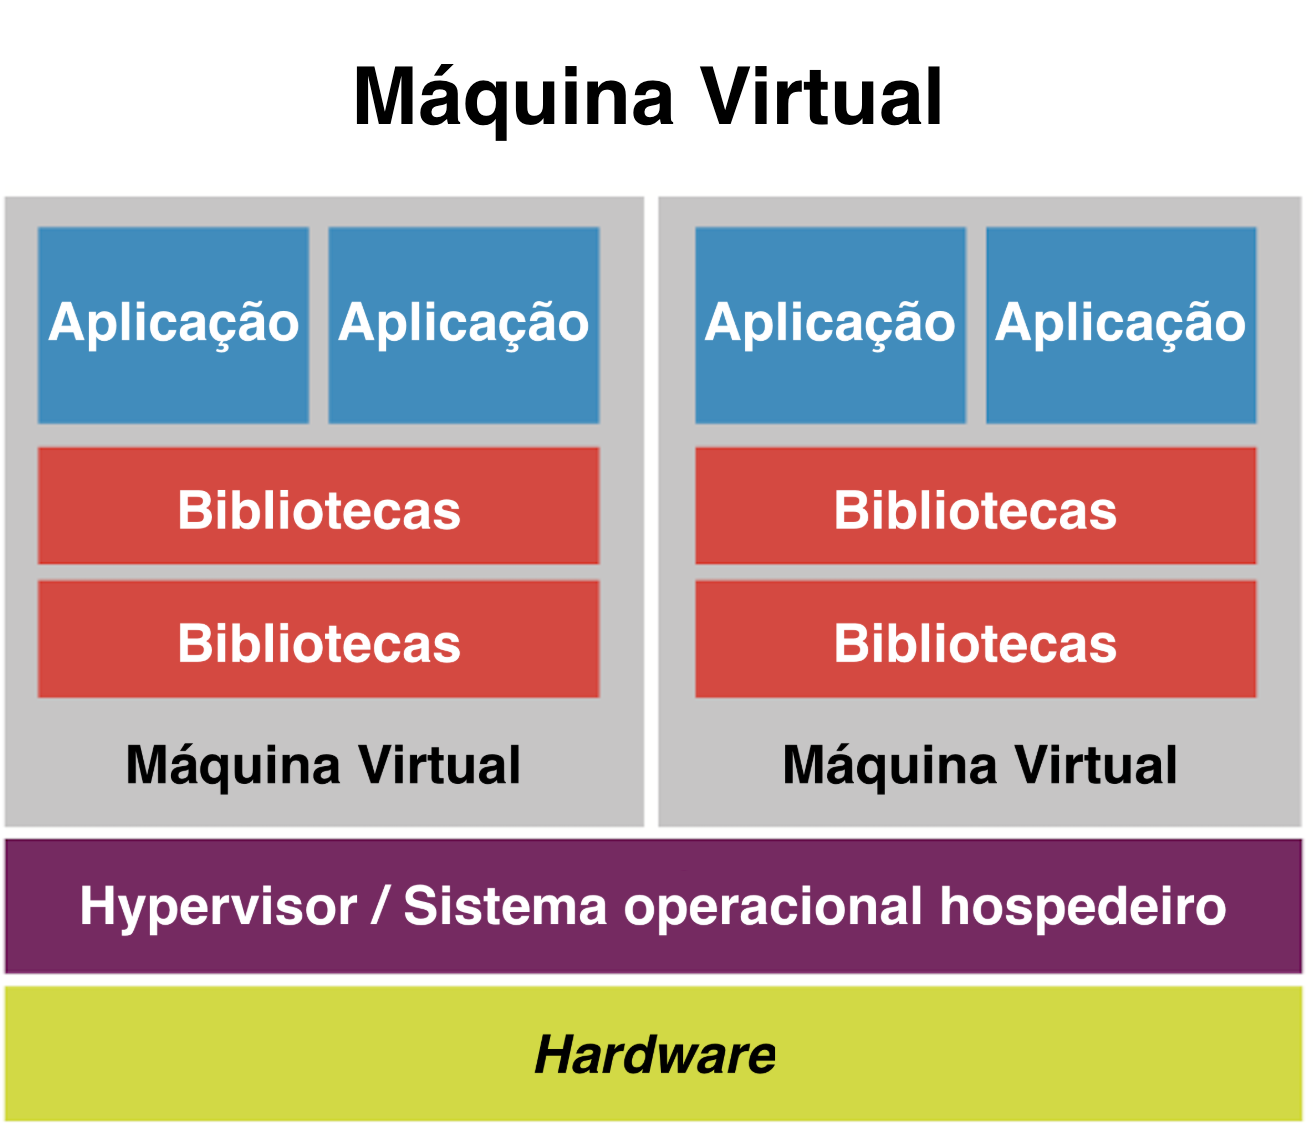
\includegraphics[width=6cm]{apresentacao/figuras/VM_Virtualization}
        
%     	Fonte: Adaptado de \cite{paascontainer}
%      	\label{virtualization_layers}
%     \end{figure}
% \end{frame}

% -------------------------------------------------%

\begin{frame}
    \centering
    \Large{Na direção da \textcolor{red}{hiperconvergência de infraestrutura}:
    \\Proposta de \textcolor{red}{armazenamento distribuído}
    \\baseado em \textcolor{red}{contêineres} para o \textcolor{red}{IFSC}}
    \break
\end{frame}

% -------------------------------------------------%

\begin{frame}
    \centering
    \Large{Na direção da \textbf{\textcolor{red}{hiperconvergência de infraestrutura}}:
    \\Proposta de \textcolor{red}{armazenamento distribuído}
    \\baseado em \textcolor{red}{contêineres} para o \textcolor{red}{IFSC}}
    \break
\end{frame}

% -------------------------------------------------%

\section{Infraestrutura hiperconvergente}

\begin{frame}{Convergência de Infraestrutura}
    \begin{block}{Convergência}
        A convergência de infraestrutura (CI) almeja alcançar o melhor desempenho do sistema com padronização dos protocolos e \textit{hardware} utilizado no \textit{data center}, muitas vezes através da utilização de \textit{hardware} proprietário que realize funções específicas \cite{netappconvergence}.
    \end{block}
    
     \begin{block}{Hiperconvergência}
        É uma infraestrutura definida por \textit{software} que pode ser dimensionada horizontalmente \cite{vmwarehyperconvergence} e que combina computação, virtualização, armazenamento e rede em um único \textit{cluster} e em uma única plataforma de gerenciamento \cite{ciscohyperconvergence}.
    \end{block}   
\end{frame}

% -------------------------------------------------%

\begin{frame}
    \centering
    \Large{Na direção da \textcolor{red}{hiperconvergência de infraestrutura}:
    \\Proposta de \textcolor{red}{armazenamento distribuído}
    \\baseado em \textbf{\textcolor{red}{contêineres}} para o \textcolor{red}{IFSC}}
    \break
\end{frame}

% -------------------------------------------------%

\section{Contêineres}

\begin{frame}{Contêineres}
    \begin{block}{Contêineres}
        Um contêiner pode ser definido como um pacote executável de um \textit{software} que inclui tudo o que é necessário para executar este \textit{software}: códigos, bibliotecas, configurações, ferramentas, entre outros \cite{aboutcontainer}.
    \end{block}
    
    \begin{block}{Tecnologias de contêineres}
    \begin{itemize}
        \item LXC
        \item LXD
        \item Docker
    \end{itemize}
    \end{block}
\end{frame}

% -------------------------------------------------%

\begin{frame}{Contêineres}
    \begin{figure}[!htpb]
    	\centering
    	\caption{Comparação entre máquinas virtuais e contêineres}
        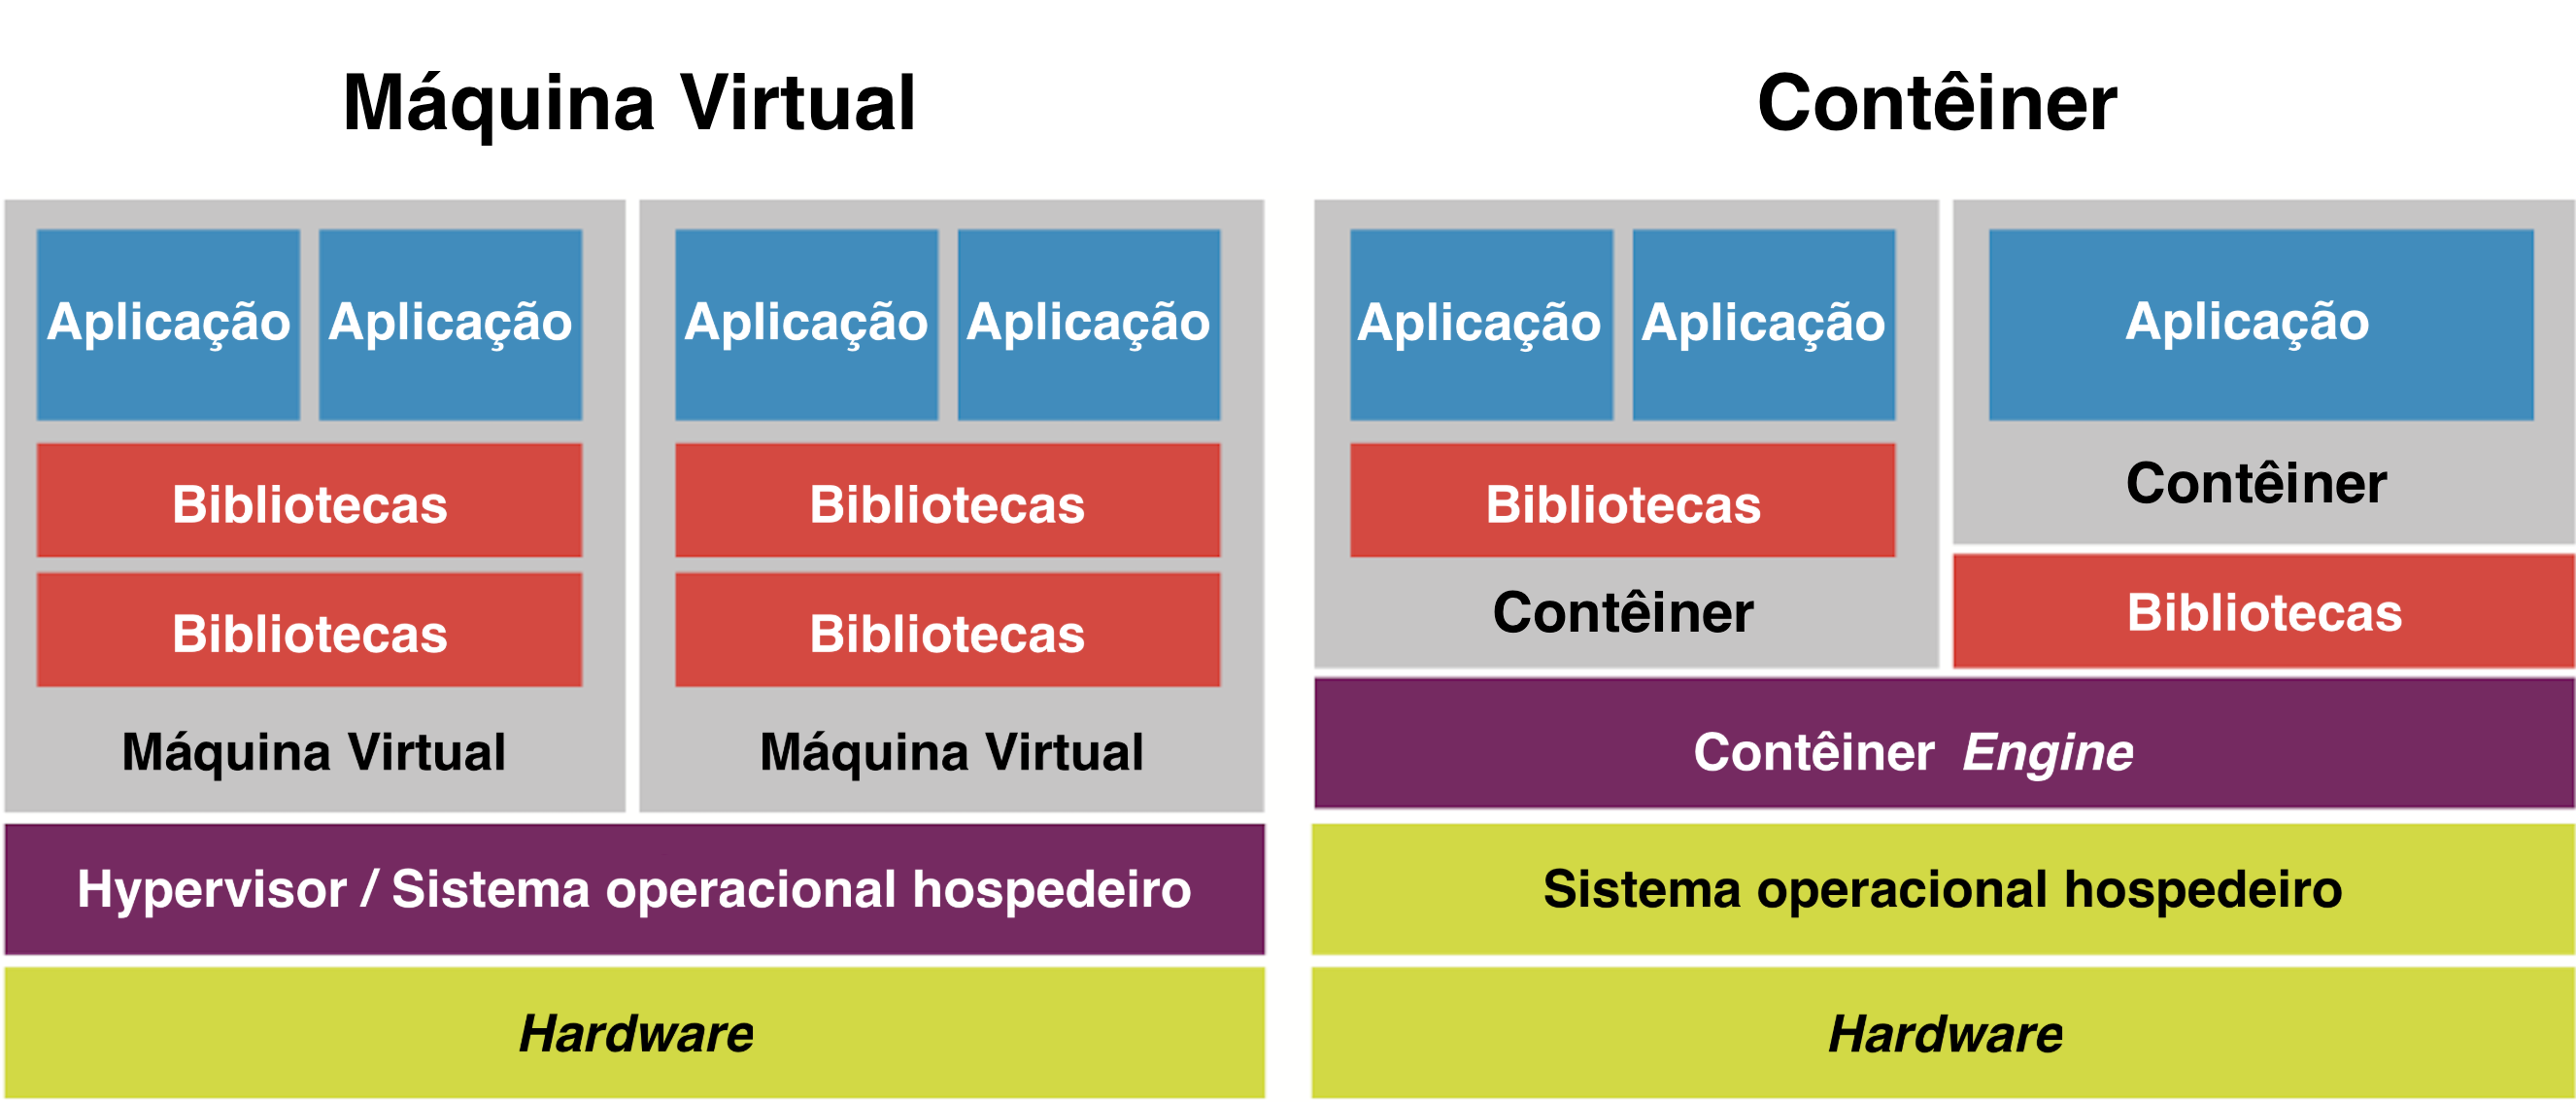
\includegraphics[width=11cm]{apresentacao/figuras/Virtualization}
        
    	Fonte: Traduzido de \cite{paascontainer}
     	\label{virtualization_layers}
    \end{figure}
\end{frame}

% -------------------------------------------------%

\begin{frame}{Orquestração de contêineres}
    \begin{block}{Orquestração de contêineres}
        Um orquestrador de contêineres é um sistema que provê um \textit{framework} para integração e gestão de contêineres em larga escala \cite{containerOrchestration}.
    \end{block}
    
    \begin{block}{Exemplos de Orquestradores}
    \begin{itemize}
        \item Docker Swarm
        \item Kubernetes
        \begin{itemize}
            \item \textit{Google Kubernetes Engine} (GKE)
            \item \textit{Amazon Elastic Container Service for Kubernetes} (EKS)
            \item \textit{Azure Kubernetes Service} (AKS)
        \end{itemize}
    \end{itemize}
    \end{block}
\end{frame}

% -------------------------------------------------%

\begin{frame}
    \centering
    \Large{Na direção da \textcolor{red}{hiperconvergência de infraestrutura}:
    \\Proposta de \textbf{\textcolor{red}{armazenamento distribuído}}
    \\baseado em \textcolor{red}{contêineres} para o \textcolor{red}{IFSC}}
    \break
\end{frame}

% -------------------------------------------------%

\section{Armazenamento distribuído}

\begin{frame}{Armazenamento distribuído}
    \begin{block}{Sistemas de armazenamento distribuído de código aberto}
        \begin{itemize}
            \item Ceph
            \item StorageOS
            \item GlusterFS
            \item Lustre
            \item ...
        \end{itemize}
    \end{block}
\end{frame}

% -------------------------------------------------%

\begin{frame}{Ceph}
    \begin{block}{Definição}
        Ceph é um sistema de armazenamento distribuído de código aberto. Este sistema de armazenamento permite que dados sejam armazenados não apenas no formato de arquivos, mas também como blocos e objetos \cite{cephdocumentation}.
    \end{block}
    
    \begin{block}{Onde o Ceph é utilizado}
    \begin{itemize}
        \item Cisco
        \item Digital Ocean
        \item Western Digital
    \end{itemize}
    \end{block}
    
    \begin{block}{Implementação do Ceph em Kubernetes}
    \begin{itemize}
        \item Rook
    \end{itemize}
    \end{block}
\end{frame}

% -------------------------------------------------%

\section{Implementação de armazenamento distribuído em infraestrutura de contêineres hiperconvergente}

\begin{frame}{Aplicação WordPress em Kubernetes}
    \begin{figure}[!htpb]
    	\centering
    	\caption{Publicação WordPress utilizando imagem armazenada como objeto no Rook}
        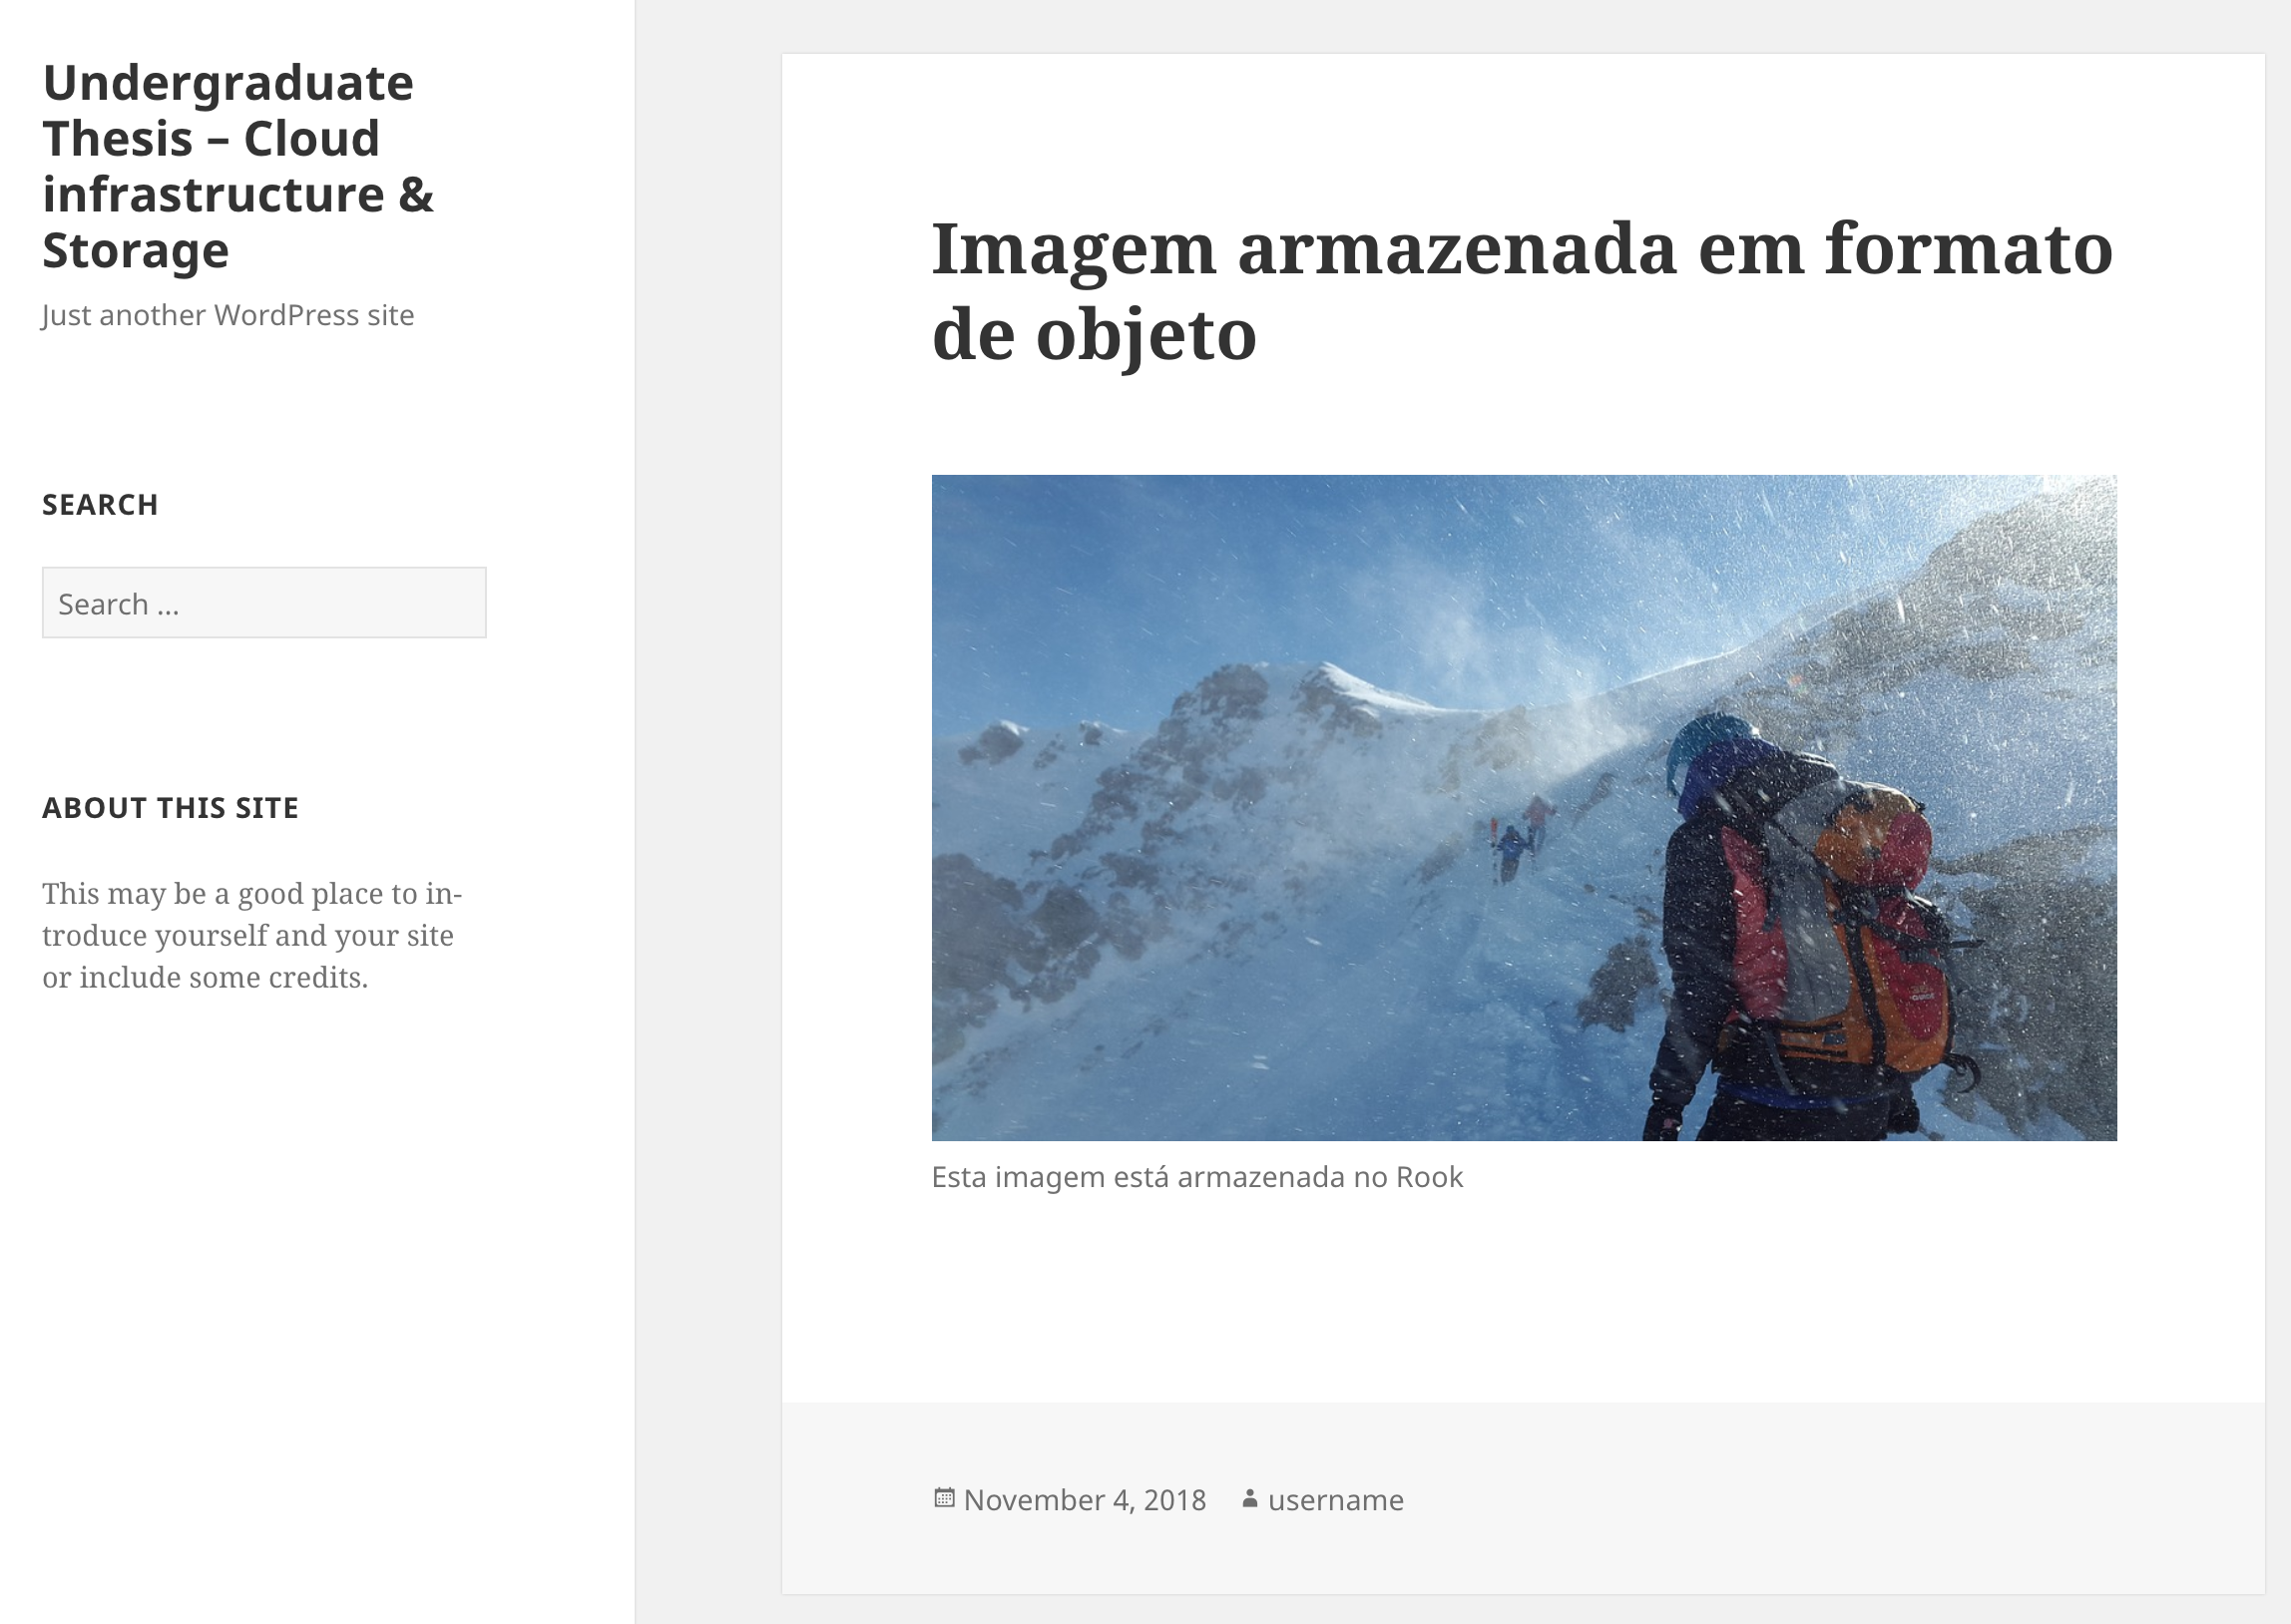
\includegraphics[width=8cm]{apresentacao/figuras/wordpress-post}
        
    	Fonte: Elaborado pelo autor.
     	\label{wordpress_post}
    \end{figure}
\end{frame}

% -------------------------------------------------%

\begin{frame}
    \centering
    \Large{Na direção da \textcolor{red}{hiperconvergência de infraestrutura}:
    \\Proposta de \textcolor{red}{armazenamento distribuído}
    \\baseado em \textcolor{red}{contêineres} para o \textbf{\textcolor{red}{IFSC}}}
    \break
\end{frame}

% -------------------------------------------------%

\section{IFSC}

\begin{frame}{IFSC}
    \begin{block}{Cenário Atual}
        \begin{itemize}
            \item Infraestrutura de serviços centralizada na Reitoria
            \item Topologia vertical
            \item Confiabilidade em \textit{hardware}
        \end{itemize}
    \end{block}
 \end{frame}

% -------------------------------------------------%

\begin{frame}{IFSC}
    \begin{block}{Cenário Ideal}
        \begin{itemize}
            \item Alta disponibilidade
            \item Baixo custo
            \item Alto poder de processamento
            \item Alta redundância e replicação de dados
        \end{itemize}
    \end{block}
\end{frame}

% -------------------------------------------------%

\begin{frame}{IFSC}
    \begin{figure}[!htpb]
    	\centering
    	\caption{Infraestrutura de serviços proposta}
        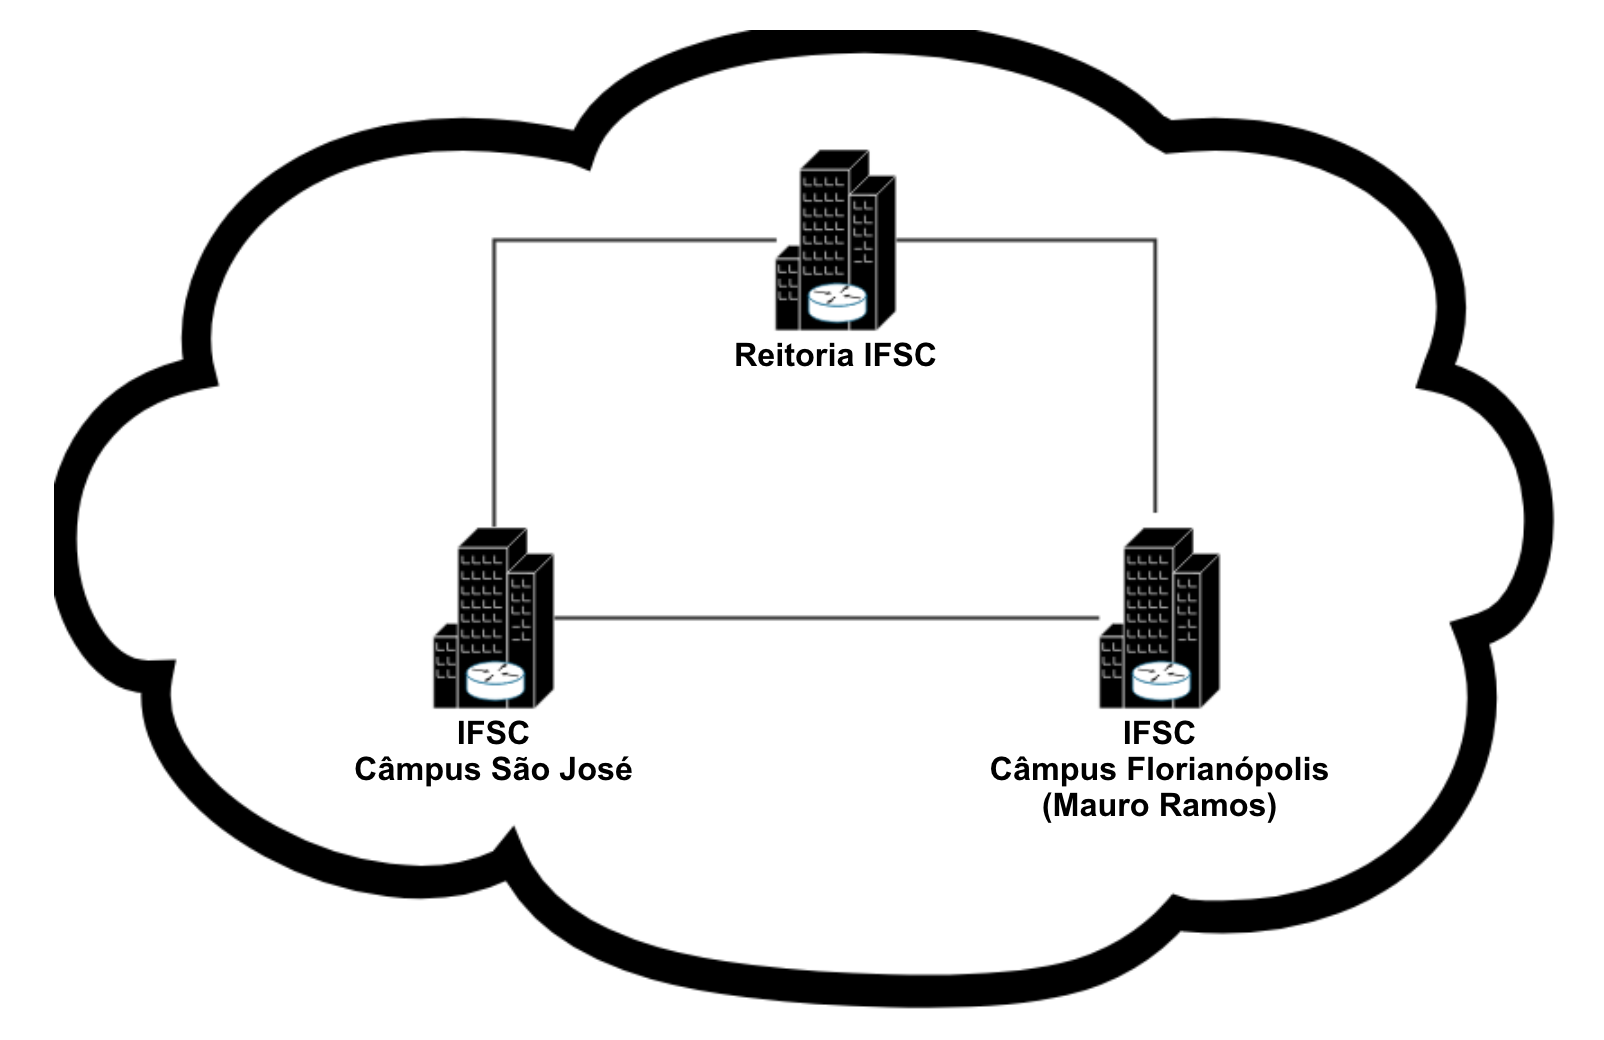
\includegraphics[width=9cm]{apresentacao/figuras/IFSC-Cloud}
        
    	Fonte: Elaborado pelo autor.
     	\label{wordpress_post}
    \end{figure}
\end{frame}

% -------------------------------------------------%

\begin{frame}{IFSC}
    \begin{block}{Infraestrutura proposta}
        \begin{itemize}
            \item Alta disponibilidade \checkmark
            \item Baixo custo \checkmark
            \item Alto poder de processamento \checkmark
            \item Alta redundância e replicação de dados \checkmark
        \end{itemize}
    \end{block}
\end{frame}

% -------------------------------------------------%

\begin{frame}{IFSC}
    \begin{figure}[!htpb]
    	\centering
    	\caption{Fluxograma de implantação da infraestrutura proposta no IFSC}
        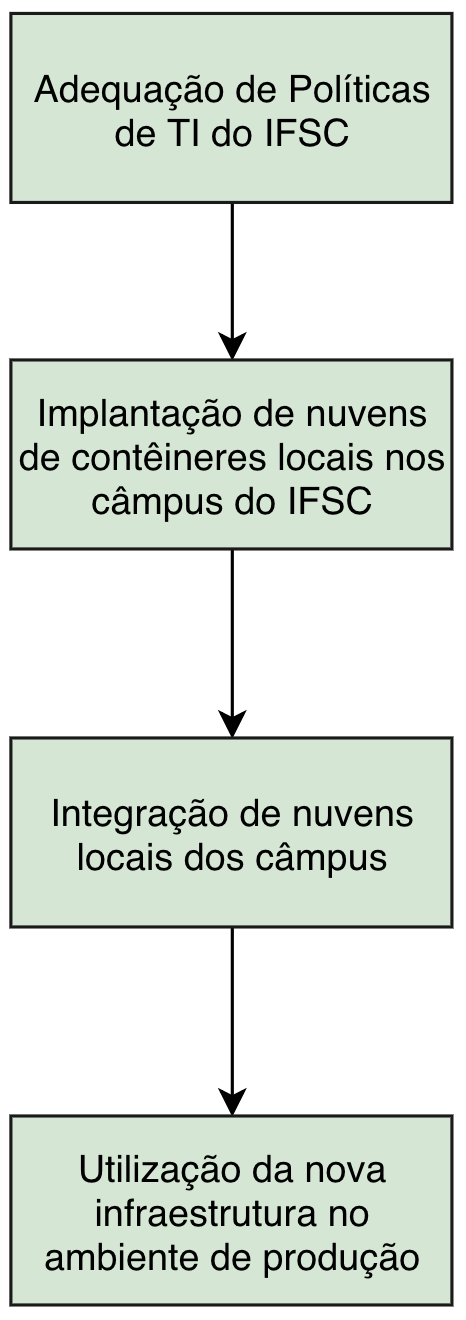
\includegraphics[height=6cm]{apresentacao/figuras/Fluxograma-Plano_IFSC}
        
    	Fonte: Elaborado pelo autor.
     	\label{wordpress_post}
    \end{figure}
\end{frame}

% -------------------------------------------------%

\begin{frame}{IFSC}
    \begin{figure}[!htpb]
    	\centering
    	\caption{Organograma simplificado dos departamentos de TIC do IFSC}
        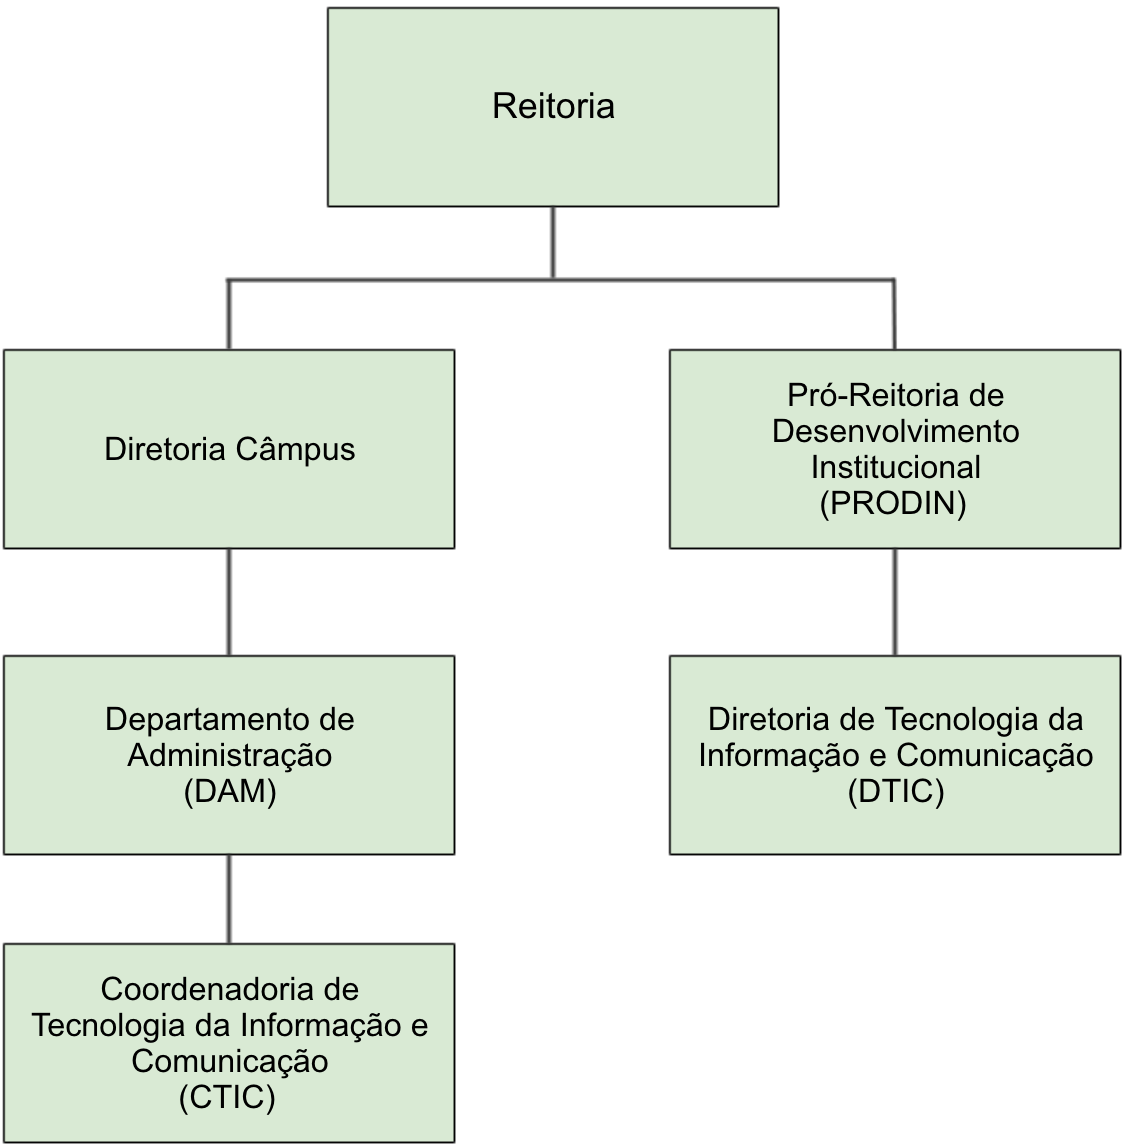
\includegraphics[height=6cm]{apresentacao/figuras/Organograma-CTIC_DTIC}
        
    	Fonte: Elaborado pelo autor.
     	\label{wordpress_post}
    \end{figure}
\end{frame}

% -------------------------------------------------%

\begin{frame}{IFSC}
    \begin{figure}[!htpb]
    	\centering
    	\caption{Fluxograma de implantação da infraestrutura proposta no IFSC}
        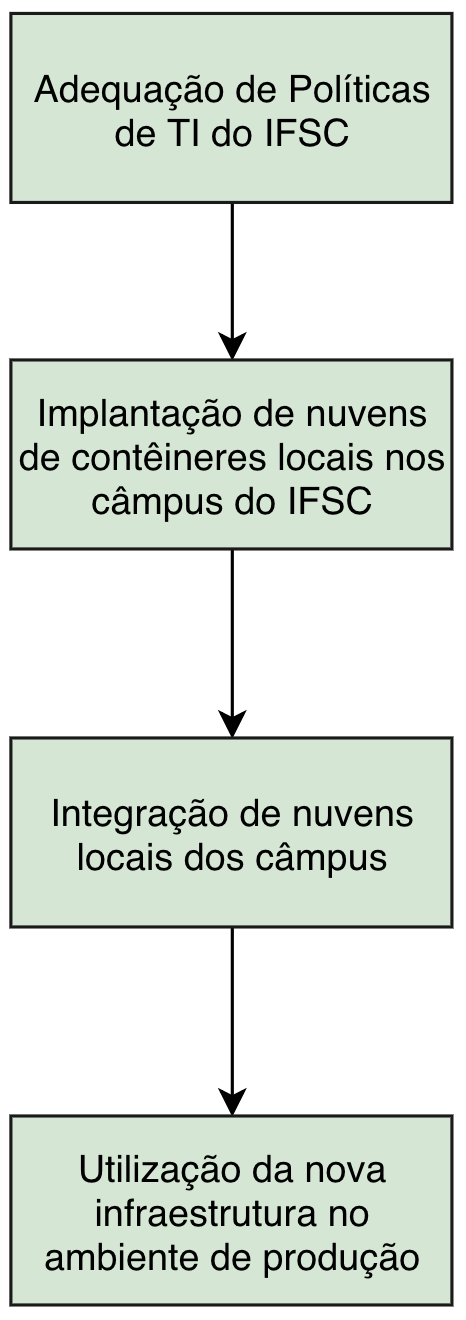
\includegraphics[height=6cm]{apresentacao/figuras/Fluxograma-Plano_IFSC}
        
    	Fonte: Elaborado pelo autor.
     	\label{wordpress_post}
    \end{figure}
\end{frame}

% -------------------------------------------------%

\section{Considerações finais}

\begin{frame}{Considerações finais}
    \begin{block}{Desafios do trabalho}
    \begin{itemize}
        \item Acesso a informação no IFSC
        \item Tecnologias emergentes e não abordadas no curso    \end{itemize}
    \end{block}
% -------------------------------------------------%
    
    \begin{block}{Conclusões}
    \begin{itemize}
        \item Desafio na implantação do sistema do ponto de vista técnico e de gestão de TI
        \item Pioneirismo na adoção de tecnologias emergentes
        \item Auxiliar ensino a distância e laboratórios remotos
    \end{itemize}
    \end{block}
\end{frame}

% -------------------------------------------------%

\begin{frame}{Trabalhos futuros}
    \begin{block}{Trabalho}
    \begin{itemize}
        \item Testes do sistema de armazenamento distribuído proposto neste trabalho em ambientes de produção do IFSC.
        \item Estudo de viabilidade de implantação de serviços atualmente utilizados pelo IFSC em uma infraestrutura de contêineres.
        \item Estudo de mecanismos de monitoramento de serviços e de infraestrutura de contêineres.
        \item Estudo de desempenho de serviços na infraestrutura de contêineres com utilização de diferente \textit{hardware} para processamento.
    \end{itemize}
    \end{block}
\end{frame}

% -------------------------------------------------%

\begin{frame}{Referências}
    \footnotesize{\bibliography{bibliografia}}
\end{frame}

\end{document}